\subsection{Unit test}
Per questa iterazione è stata testata la funzione findById presente nel backend, che serve a recuperare un evento tramite id.

\begin{lstlisting}
@DataJpaTest
class EventRepositoryTest {

	@Autowired
	private EventRepository underTest;
	
	@Test
	void findById() {
			
	String stringaTest = "test";
	//given
	Date date = new Date(100);
	Event expected = new Event(stringaTest, stringaTest, 
	EventLevel.MEDIUM, date, stringaTest, stringaTest, 
	stringaTest, stringaTest, stringaTest, stringaTest, 
	stringaTest, new Integer(4));
	underTest.save(expected);
	
	//when
	Event result = underTest.findById(expected.getId()).get();
	
	//then
	assertThat(expected.getDescription())
	.isEqualTo(result.getDescription());
	}
}
\end{lstlisting}

\begin{figure}[h!]
\begin{center}
  % Requires \usepackage{graphicx}

  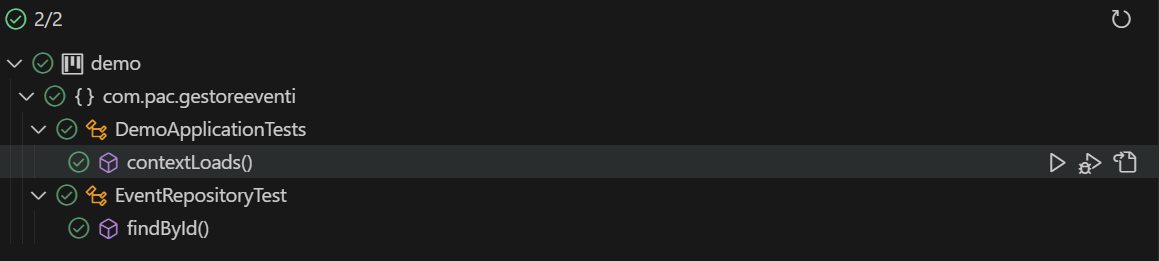
\includegraphics[width=16cm]{test/unit test/unit.PNG}\\
  \caption{findById()}
\end{center}
\end{figure}
